\chapter{Implementacja aplikacji}

\section{Architektura}
Aplikacja została stworzona w języku C++ oraz wykorzystuje elementy obiektowe tego języka programowania. Klasy projektu przedstawione są na diagramie 8.1.\\
\begin{figure}[h]
\centering
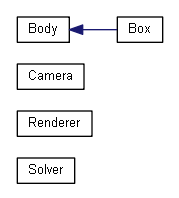
\includegraphics[width=0.3\textwidth]{figures/classes.png}
\caption{Diagram klas (opracowanie własne).}%
\label{rys:Podzial klas}
\end{figure}
Plik nagłówkowy \verb$stdafx.h$ zawiera informacje o wszystkich dołączonych do projektu plikach źródłowych, bibliotek oraz zdefiniowane stałe. Dzięki wykorzystaniu takiego rozwiązania możliwe jest łatwe zarządzanie projektem oraz zmniejszone jest ryzyko błędu wielokrotnego dołączania tej samej biblioteki lub pliku źródłowego.\\
Plik \verb$main.cpp$ zawiera inicjalizację instancji klas odpowiedzialnych za renderowanie oraz komunikację z układem GPU. Tworzone są tu również obiekty symulacji. Znajduje się tutaj również główna pętla aplikacji.\\
Klasa \verb$Camera$ zawiera implementację uproszczonej kamery, umożliwiającej poruszanie się po renderowanej scenie.
\verb$Renderer$ odpowiada za stworzenie okna aplikacji, ciągłe generowanie obrazu symulowanych brył, przemieszczanie kamery oraz przełączanie trybu pomiędzy wyswietlaniem brył oraz samych ich siatek.
Klasa \verb$Solver$ obejmuje komunikację z GPU oraz posiada implementację obliczeń fizycznych wykorzystujących CPU.
Klasa \verb$Renderer$, \verb$Solver$ oraz \verb$Camera$ zostały stworzone wykorzystując wzorzec projektowy Singleton\footnote{Singleton - kreacyjny wzorzec projektowy. Gwarantuje, że klasa będzie miała tylko jeden egzemplarz i zapewnia globalny dostęp do niego\cite{Wzorce projektowe}.}. Celem zastosowania wzorca jest ograniczenie liczby stworzonych instancji danej klasy do jednej oraz zapewnienie globalnego dostępu do stworzonego obiektu. W przypadku każdej klasy korzystającej z tego wzorca, implementacja sprowadza się do stworzenia statycznej metody zwracającej referencję do instancji obiektu. Wywoływana metoda dodatkowo tworzy obiekt klasy przy pierwszym jej uzyciu. Należy pamiętać, aby zarówno kontruktor jak i instancja klasy były składowymi prywatnymi, aby uniemożliwić stworzenie większej ilości obiektów danej klasy.\\
\verb$Body$ jest klasą bazową, zawierającą strukturę obiektu, metody ustawiające, pobierające oraz obliczające odpowiednie elementy struktury.
\verb$Box$ jest klasą dziedziczącą po klasie \verb$Body$. Ustawia ona typ tworzonej bryły oraz nadpisuje część metod obliczających z klasy bazowej.
Dodatkowo plik \verb$Phys.cl$ zawierający logikę obliczanych sił oraz przemieszczeń obiektów na~urządzeniu GPU.

\section{Struktury danych}
Ważnym elementem aplikacji jest struktura \verb$myBody$ zawarta w klasie \verb$Body$. Zawiera ona następujace dane:
\begin{itemize}
\item center -  centralny punkt obiektu w postaci trzech wartości typu zmiennoprzecinowego, odzwierciedlających położenie w globalnej przestrzeni trójwymiarowe,
\item lengths - długości odcinków od środka obiektu do jego krawędzi prowadzonych wzdłuż lokalnych osi układu współrzędnych,
\item velocity - aktualna wartość wektora prędkości,
\item angularVelocity - aktualna wartość wektora prędkości kątowej obiektu wyrażona w~postaci trzech liczb,
\item weight - masa bryły,
\item orientation - aktualny obrót obiektu wyrażony w postaci kwaternionu,
\item isActive - zmienna binarna określająca stan obiektu,
\item type - zmienna wskazująca na typ bryły,
\item points - obliczone współrzędne wierzchołków, służące do poprawnego wyrenderowania bryły.
\end{itemize}
Identyczna struktura znajduje się w pliku \verb$Phys.cl$. Położenie kolejnych elementów struktury zarówno w pliku kernela jak i pliku klasy musi być identyczne, gdyż w innym przypadku, np. zamieniając w strukturze kernela miejscami pola center oraz lengths, wartości używane od obliczeń byłyby zmienione i powodowałyby błędne wyniki.

\section{Przesyłanie danych między CPU a GPU}
Idea przesyłania danych pomiędzy pamięcią RAM a pamięcią urządzenia GPU została opisana w rozdziale siódmym. Po utworzeniu kontekstu oraz kolejki zadań, stworzony jest bufor o wielkości równej pamięci potrzebnej na przechowanie struktury dla jednej bryły pomnożonej przez liczbę brył biorących udział w symulacji. Dostęp do bufora jest typu CL\_MEM\_READ\_WRITE, co oznacza, iż możliwe jest zarówno odczytywanie jak i~zapisywanie do niego danych. Następnie uzupełniane są argumenty przesyłane do funkcji kernela:
\begin{itemize}
\item wkaźnik na bufor obiektów,
\item liczba obiektów biorących udział w symulacji,
\item czas, jaki upłynął pomiędzy kolejnymi iteracjami pętli.
\end{itemize}
Po wykonaniu operacji należy przekopiować z powrotem dane z bufora do listy obiektów. Umożliwienie zarówno odczytu jak i zapisu do jednego bufora pozwoliło zmniejszyć zapotrzebowanie na pamięć układu GPU. Aby jednak było to możliwe, operacje wykonywane na~danych znajdujących się w buforze musiały zostać zaimplementowane w taki sposób, by nie ingerować w elementy struktury wykorzystywane do sprawdzania kolizji z innymi bryłami.